%
% $Id: $
%
%
% Compilar a .pdf con LaTeX (pdflatex)
% Es necesario instalar Beamer (paquete latex-beamer en Debian)
%

%
% Gr�ficos:
% Los gr�ficos pueden suministrarse en PNG, JPG, TIF, PDF, MPS
% Los EPS deben convertirse a PDF (usar epstopdf)
%

\documentclass{beamer}
\usetheme{Warsaw}
%\usebackgroundtemplate{
\includegraphics[width=\paperwidth]{format/libresoft-bg.png}}
%\usepackage[spanish]{babel}
\usepackage[latin1]{inputenc}
\usepackage{graphics}
\usepackage{amssymb} % Simbolos matematicos
\usepackage{url}
\usepackage{multirow}
\usepackage{hyperref}


%\definecolor{libresoftgreen}{RGB}{162,190,43}
%\definecolor{libresoftblue}{RGB}{0,98,143}

%\setbeamercolor{titlelike}{bg=libresoftgreen}

%% Metadatos del PDF.
\hypersetup{
  pdftitle={How social are Scratch learners? A comprehensive analysis of the Scratch platform for social interactions},
  pdfauthor={J. Moreno-Le�n, Gregorio Robles, Marcos Rom�n-Gonz�lez},
  pdfcreator={GSyC/LibreSoft \\ Universidad Rey Juan Carlos},
  pdfproducer=PDFLaTeX,
  pdfsubject={Code to learn with Scratch},
}
%%

\begin{document}

\title{How social are Scratch learners?}
\subtitle{A comprehensive analysis of the Scratch platform for social interactions}
\institute{jesus.moreno@programamos.es, grex@gsyc.urjc.es, mroman@edu.uned.es \\
GSyC/Libresoft, Universidad Rey Juan Carlos}
\author{J. Moreno-Le�n, Gregorio Robles, Marcos Rom�n-Gonz�lez}
\date{FLOSSEdu workshop @ OSS 2016, Gothenburg, June 2\textsuperscript{nd} 2016}

\frame{
\maketitle
\begin{center}

\includegraphics[width=2cm]{format/libresoft-logo}
\hspace{0.5cm}

\includegraphics[width=5cm]{format/gsyc-urjc}
\vspace{0.5cm}

\includegraphics[width=3cm]{format/emadrid.png}
\end{center}
}


% Si el titulo o el autor se quieren acortar para los pies de p�gina
% se pueden redefinir aqu�:
%\title{Titulo corto}
%\author{Autores abreviado}

%% LICENCIA DE REDISTRIBUCION DE LAS TRANSPAS
\frame{
~
\vspace{3cm}

\begin{flushright}

\includegraphics[width=2.2cm]{figs/by-sa}

{\tiny
(cc) 2016 J. Moreno-Le�n, Gregorio Robles and Marcos Rom�n-Gonz�lez\\
  Some rights reserved. This work licensed under Creative Commons \\
  Attribution-ShareAlike License. To view a copy of full license, see \\
  http://creativecommons.org/licenses/by-sa/3.0/ or write to \\
  Creative Commons, 559 Nathan Abbott Way, Stanford, \\
  California 94305, USA. \\
\ \\
Some of the figures have been taken from the Internet \\
Source, and author and licence if known, is specified. \\
For those images, \emph{fair use} applies.
}
\end{flushright}
}
%%

\section{FLOSSEdu workshop @ OSS 2016, Gothenburg}


%--------------------------------------------------------
\usebackgroundtemplate{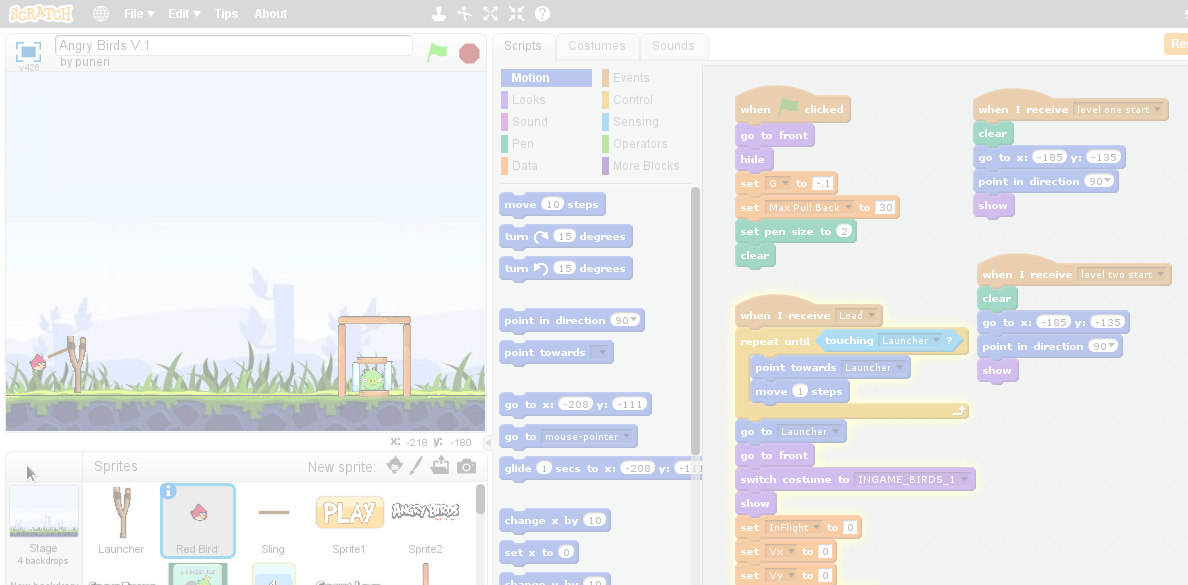
\includegraphics[width=18cm]{figs/AngryBirds2.png}}
\begin{frame}
\frametitle{Scratch}

\begin{columns}[T]
  \begin{column}{1\textwidth}
     \begin{block}{Visual programming language based on blocks}
       \begin{itemize}
         \item Designed for young learners 
         \item Massively used worldwide: 12 million users, 15 million projects
	 \item Website to share, study and remix projects, post comments or work in teams
	 \item Social aspects of sw development of FLOSS movements
       \end{itemize}
    \end{block}
  \end{column}
\end{columns}
\vspace{\baselineskip}
\hfill{\Tiny See \href{https://scratch.mit.edu/statistics/}{https://scratch.mit.edu/statistics/}}

\end{frame}
\usebackgroundtemplate{}
%--------------------------------------------------------
\usebackgroundtemplate{
\includegraphics[width=14cm]{figs/goals.jpg}}
%https://rebel-performance.com/wp-content/uploads/2014/10/goals.jpg

\begin{frame}
\frametitle{Research question}
\center{ \Large  {\bf RQ: How 'social' is the Scratch community in terms of number of comments, friends, favorites and galleries?}\\}
\vspace{\baselineskip}
\vspace{\baselineskip}
\hfill{\Tiny Background picture: rebel-performance.com}
\end{frame}

\usebackgroundtemplate{}
%--------------------------------------------------------
%--------------------------------------------------------

\begin{frame}
\frametitle{Dataset}
\begin{columns}[T]
    \begin{column}{0.5\textwidth} 
     \begin{block}{Scratch Research Data}
       \begin{itemize}
         \item Data from the Scratch online community website
         \item First five years of data, roughly 2007-2012
	 \item Core datasets, Text and Code datasets and Project Analytics datasets
       \end{itemize}
     \end{block}
    \end{column}
    \begin{column}{0.5\textwidth}
     \begin{block}{Core Dataset}
       \begin{itemize}
        \item 1,056,951 users
        \item 1,928,699 projects
        \item 120,097 galleries
        \item 1,313,200 friends
        \item 1,041,387 favorites
        \item 7,788,414 project comments
       \end{itemize}
     \end{block}
    \end{column}
  \end{columns}
\end{frame}

\usebackgroundtemplate{}
%------------------------------------------------------------

\begin{frame}
\frametitle{Results (I)}
\begin{center}
	\begin{figure}[t!]
		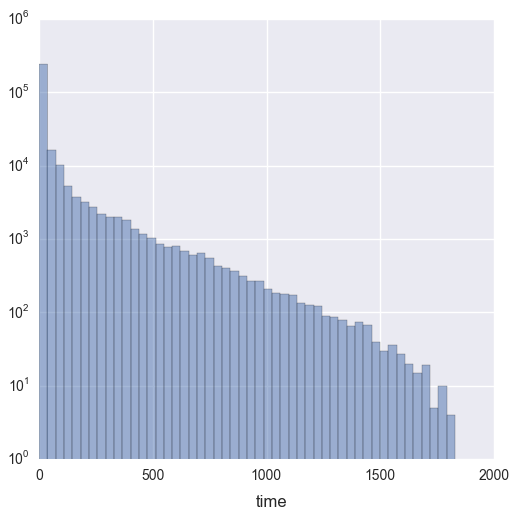
\includegraphics[width=6.5cm]{figs/time.png}    
    		\caption{Distribution of users in terms of time (days) in the community.}
	\end{figure}
\end{center}

\end{frame}

\usebackgroundtemplate{}

%------------------------------------------------------------

\begin{frame}
\frametitle{Results (II)}
\begin{center}
	\begin{figure}[t!]
		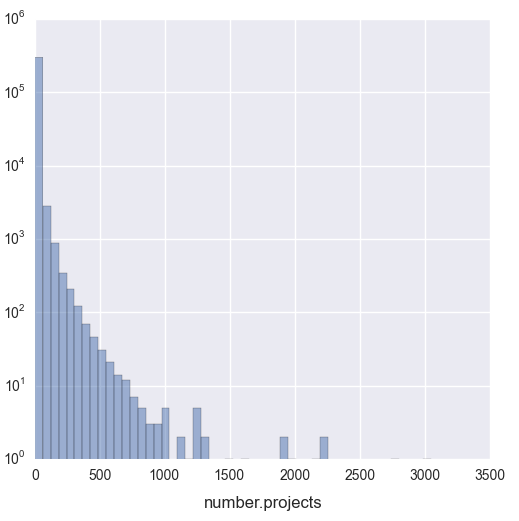
\includegraphics[width=6.5cm]{figs/nprojects.png}    
    		\caption{Distribution of users in terms of number of published projects.}
	\end{figure}
\end{center}

\end{frame}

\usebackgroundtemplate{}

%------------------------------------------------------------

\begin{frame}
\frametitle{Results (III)}
\begin{center}
	\begin{figure}[t!]
		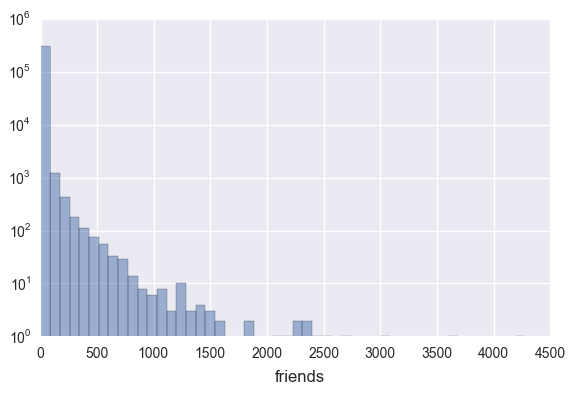
\includegraphics[width=7.5cm]{figs/friends.png}    
    		\caption{Distribution of users in terms of number of friends.}
	\end{figure}
\end{center}

\end{frame}

\usebackgroundtemplate{}

%------------------------------------------------------------

\begin{frame}
\frametitle{Results (IV)}
\begin{center}
	\begin{figure}[t!]
		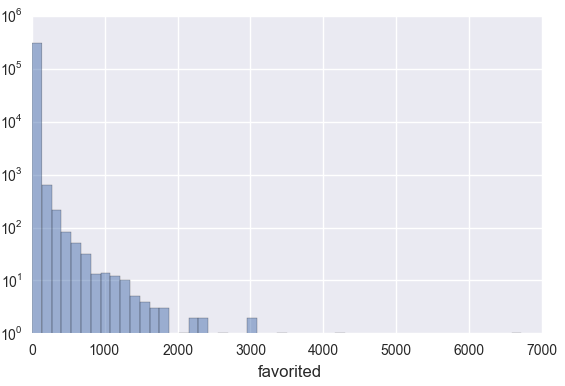
\includegraphics[width=7.5cm]{figs/favs.png}    
    		\caption{Distribution of users in terms of number of favorites.}
	\end{figure}
\end{center}

\end{frame}

\usebackgroundtemplate{}

%------------------------------------------------------------

\begin{frame}
\frametitle{Results (V)}
\begin{center}
	\begin{figure}[t!]
		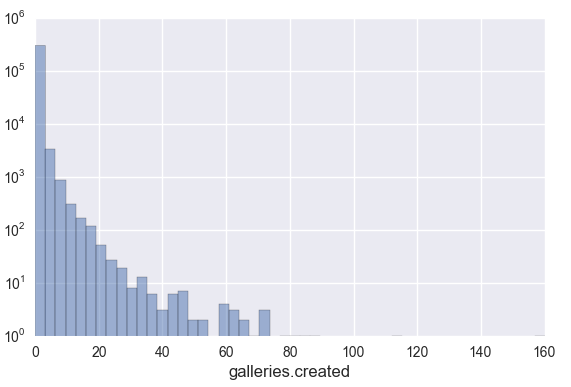
\includegraphics[width=7.5cm]{figs/galleries.png}    
    		\caption{Distribution of users in terms of number of galleries created.}
	\end{figure}
\end{center}

\end{frame}

\usebackgroundtemplate{}

%------------------------------------------------------------

\begin{frame}
\frametitle{Results (VI)}
\begin{center}
	\begin{figure}[t!]
		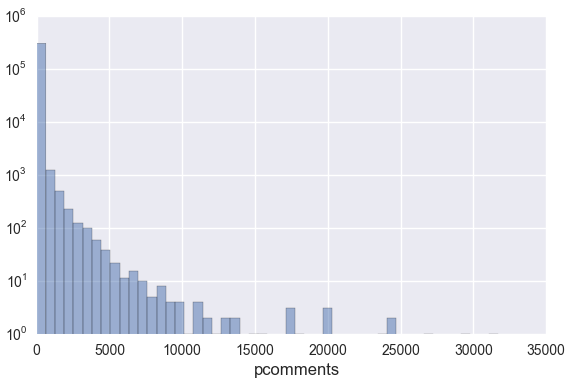
\includegraphics[width=7.5cm]{figs/pcomments.png}    
    		\caption{Distribution of users in terms of number of comments posted in project pages.}
	\end{figure}
\end{center}

\end{frame}

\usebackgroundtemplate{}

%------------------------------------------------------------

\begin{frame}
\frametitle{Results (VII)}
\begin{table}[h!]
\centering
\caption{Social activities of users with at least 5 published projects.}
\label{table:social5}
\begin{tabular}{lcccc}
\hline
     & Galleries & Friends & Favorited & Comments \\ \hline
Mean & 0.94 & 12.72 & 11.42 & 100.05 \\
Std  & 2.55 & 65.33 & 69.30 & 538.75 \\
10\% & 0    & 0     & 0 & 0 \\
20\% & 0    & 0    & 0 & 0 \\
30\% & 0    & 0    & 0 & 0 \\
40\% & 0    & 0    & 0 & 2 \\
50\% & 0    & 1    & 0 & 5 \\
60\% & 0    & 2    & 1 & 10 \\
70\% & 1    & 4    & 3 & 21 \\
80\% & 1    & 8    & 7 & 49 \\
90\% & 3    & 21   & 19 & 161 \\
100\% & 160 & 4,281 & 6,721 & 31,669 \\ \hline
\end{tabular}
\end{table}

\end{frame}

%------------------------------------------------------------

\begin{frame}
\frametitle{Results (and VIII)}
\begin{table}[h!]
\centering
\caption{Characteristics of projects in collaborative galleries and projects not in them.}
\label{table:collab}
\begin{tabular}{lcc}
\hline
 & Not in collab gallery & In collab gallery \\ \hline
n & 1,469,386 & 459,313 \\
Blocks & 100.84 & 152.24 \\
Type of blocks & 12.44 & 14.31\\
Costumes & 17.20 & 25.84 \\
Sounds & 3.75 & 4.86 \\
Ugstrings & 36.15 & 55.01\\ \hline
\end{tabular}
\end{table}

\end{frame}

\usebackgroundtemplate{}

%--------------------------------------------------------

\usebackgroundtemplate{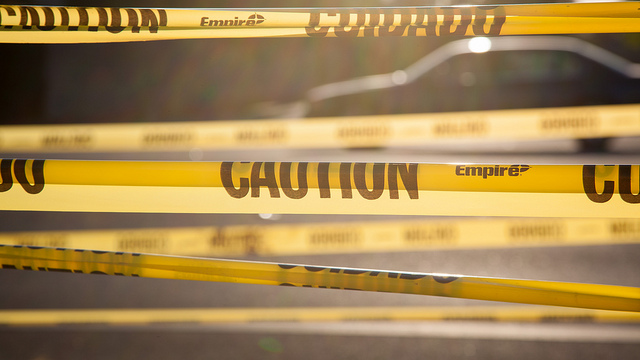
\includegraphics[width=16cm]{figs/caution.jpg}}
% background: http://25.media.tumblr.com/b83aa72682992ab34b8ce7e61c0cb7f9/tumblr_menxc7qcq61ryin08o1_r1_1280.jpg

\begin{frame}
\frametitle{Limitations}
\begin{columns}[T]
  \begin{column}{0.8\textwidth}
    \begin{block}{Several aspects must be taken into account}
      \begin{itemize}
        \item Data from 2007-2012, old version of the Scratch website (\footnotesize see \href{http://web.archive.org/web/20080527194722/http://scratch.mit.edu/}{Internet archive})
        \item \normalsize Since 2012, important modifications in the website to enhance users' social participation
        \item Study limited to online activities. Other social actions performed in offline contexts (helping a peer, working in teams) are out of the scope of the investigation.
      \end{itemize}
    \end{block}
  \end{column}
\end{columns}
\vspace{\baselineskip}
\vspace{\baselineskip}
\hfill{\Tiny Background picture:  Robert Couse-Baker}
\end{frame}

\usebackgroundtemplate{}

%-----------------------    ---------------------------------
\usebackgroundtemplate{
\includegraphics[width=13cm]{figs/take-away.jpg}}
%% background: http://flamingcow.co.uk/wp-content/uploads/2015/02/takeaway-940x283.jpg
\begin{frame}
\frametitle{Conclusions}
\begin{itemize}
	\item \textbf{The vast majority of Scratch users barely make use of the social capabilities offered by the website.}
	\item Medians of users who have published at least five projects:
	\begin{itemize}
	  \item 1 friend
	  \item 5 comments
	  \item 0 galleries
	  \item 0 favorites
	\end{itemize}
\end{itemize}

\hfill{\Tiny Background picture: flamingcow.co.uk}
\end{frame}

\usebackgroundtemplate{}

%--------------------------------------------------------
\usebackgroundtemplate{
\includegraphics[width=13cm]{figs/future.png}}

\begin{frame}
\frametitle{Future Work}

\begin{enumerate}
  \item Compare this level of activity with other social, coding communities (like Github).
  \item Analyze the impact of social participation in the learning of programming skills.
  \begin{itemize}
   \item Adaptation of Dr. Scratch to measure computational thinking skills with the information of the dataset. (\footnotesize See \href{http://drscratch.org}{http://drscratch.org})
  \end{itemize}
  \item \normalsize Access to a new dataset with more recent information would allow to perform new investigations that could yield different conclusions.
\end{enumerate}
\vspace{\baselineskip}
\vspace{\baselineskip}
\hfill{\Tiny Background picture: Simon Cunningham }

\end{frame}

\usebackgroundtemplate{}
%%--------------------------------------------------------

\frame{
\maketitle
\begin{center}

\includegraphics[width=2cm]{format/libresoft-logo}
\hspace{0.5cm}

\includegraphics[width=5cm]{format/gsyc-urjc}
\vspace{0.5cm}

\includegraphics[width=3cm]{format/emadrid.png}
\end{center}
}

\end{document}
